% NCR design with necessary equipment and point layout (wired and wireless)
% - Prepare design, identify network equipment and specifications for LAN socket point wiring.
% - Develop BoQ 
% - Your work shall consider backbone network if required, LAN socket point (wired and wireless) and NCR setup/design with cabling/ducting etc..
% -
% (Furniture layout) for group number = 8 % 8 + 1 = 1
\documentclass[12pt]{article}


\usepackage[utf8]{inputenc}
\usepackage[a4paper,top=3cm,bottom=2cm,left=3cm,right=3cm,marginparwidth=1.75cm]{geometry}
\usepackage[nodayofweek]{datetime}
\usepackage{tabularx}
\usepackage[small]{titlesec}
\usepackage{graphicx}
\usepackage{tabularx}
\usepackage{pdfpages}
\newcolumntype{L}[1]{>{\raggedright\arraybackslash}p{#1}}
\newcolumntype{C}[1]{>{\centering\arraybackslash}p{#1}}
\newcolumntype{R}[1]{>{\raggedleft\arraybackslash}p{#1}}

\begin{document}

\begin{titlepage}
    \begin{center}
        \huge{\bfseries  Tribhuvan University}\\
        \Large{Institute of Engineering}\\
        \huge{ \bfseries  Pulchowk Campus}\\[3.2cm]


        \textsc{\Large Internet and Intranet}\\[-0.5cm]
        \line(1,0){400}\\
        \huge{\bfseries Lab 5}\\
        \large{Network Specialist Tasks \\ Task = 8(Group Number)\% 8 + 1 = 1  }
        \line(1,0){400}\\


        \textsc{\Large Submitted by:}\\
        \Large Aayush Lamichhane\\ \large 075BCT005\\   [0.85cm]
        \Large Bishal Katuwal\\ \large 075BCT028\\   [0.85cm]
        \Large Bishant Baniya\\ \large 075BCT030\\   [0.85cm]
        \Large Gobind Prasad Sah\\ \large 075BCT038\\ Project Group 8\\   [0.85cm]
        \textsc{\Large Submitted to:}\\\
        \large Department of Electronics and Computer Engineering\\Pulchowk Campus\\    [0.85cm]
        
        \textsc{\Large Submitted on:}\\
        \today
        
    \end{center}
\end{titlepage}
\pagebreak
% ===============================================================
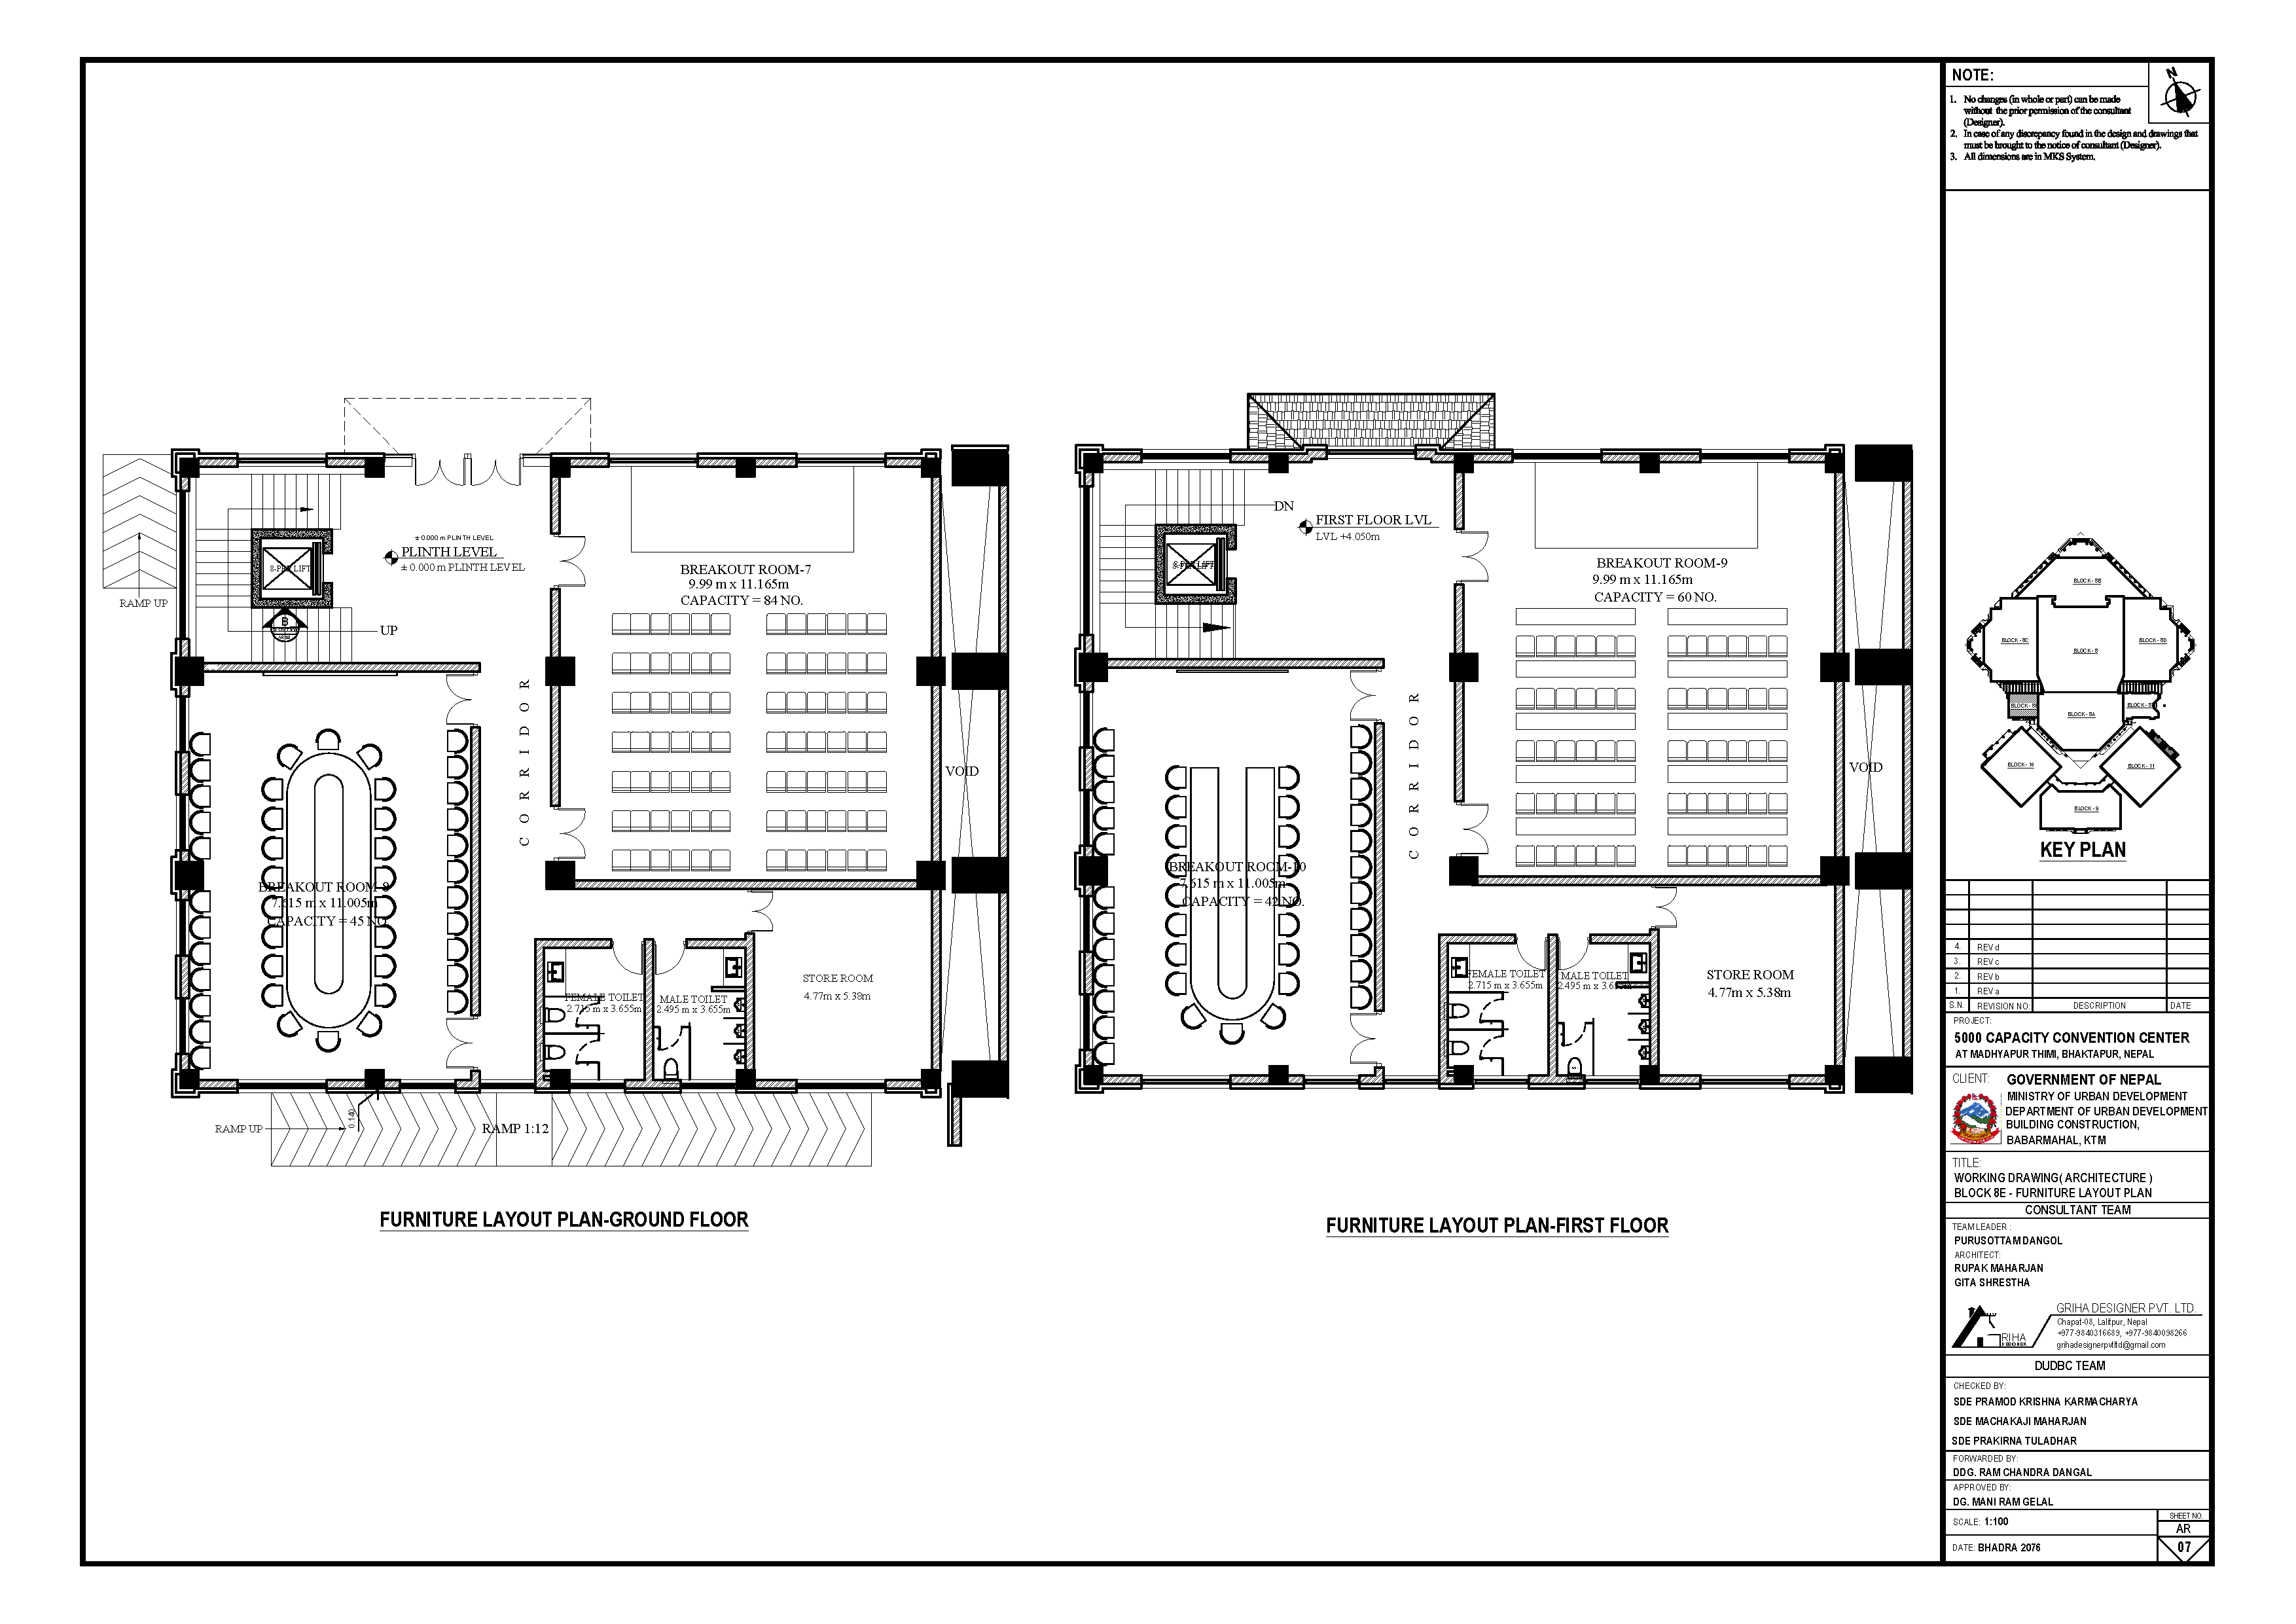
\includepdf{FurnitureLayout.pdf}
\tableofcontents
\pagebreak

\section{Introduction}
This lab report outlines the requirements for adding a network plan to block 8E of
a convention centre with an existing backbone network and Network Control Room.
The backbone and Network Control Room is considered to existing within the premises
of the building. 
The project under consideration involves the installation of all the necessary 
equipments for the said block and its integration with the backbone network. 
The connection of new network to backbone also includes a connection to the building's
Network Control Room.  
All audio-video control and management for the entire building 
is also considered to be handled from the NCR.

\section{Assumptions}
\begin{itemize}
    \item Backbone network and Network Control Room already exists.
    \item There is a fibre ring connection throughout the blocks with a terminal in block 8E which can be accessed.
    \item All audio-video recording and managementis done by NCR and not in block.
    \item Following factors are considered :
    \begin{itemize}
        \item Space
        \item equipments
        \item Cable management
        \item Accessibility
    \end{itemize} 
    \item Following factors are ignored : 
    \begin{itemize}
        \item Cooling and Ventilation
        \item Security
    \end{itemize}
\end{itemize}

\section{Scope of Project}
\begin{enumerate}
    \item Estimation of all networking devices, cabling, and face plates required for the project.
    \item Provision of a reliable and efficient networking system that meets the needs of the building occupants.
    \item Cable management system (fiber optic, UTP)
    \item identification of all the cables and termination locations.
\end{enumerate}

\section{Analysis of Network Requirements}
Assuming the building will follow the same plan upwards, the requirement for each floor is defined by:
\begin{enumerate}
\item {\bfseries The dimension of the centre and rooms \\}
Based on the layout of the building, on each floor there will be:
\begin{itemize}
    \item 2x2 breakout rooms in total
    \item 2x1 Bathrooms  
    \item 2x1 Storerooms 
    \item Ramps
\end{itemize}

\item {\bfseries The number of users and devices that will be accessing the network\\}
The capacity of breakout rooms are 84, 45, 60 and 42 respectively.

\item {\bfseries The types of data that will be transmitted\\}
The network infrastructure is designed to accommodate the different types of data that will be transmitted, including audio, video, and data files.

\item {\bfseries The desired network performance levels\\}
Tthe breakout rooms need robust connection whereas other areas can work with a slower/weaker connection.
\end{enumerate}

\section{Project Requirement Analysis}
\begin{enumerate}
    \item Workmanship: Work should be properly done by mechanic who is skilled in the trade. Engineer shall point out the defects if they exist, it shall be fixed without extra cost.
    \item Material quantity and rate (IN BOQ):
    \begin{itemize}
        \item  Information outlet 
        \item Intelligent door control system 
        \item IP telephone 
        \item CCTV system 
        \item Wireless AP 
        \item Socket-point wiring 
        \item End access POE switch
    \end{itemize}
   
\end{enumerate}

\section{Project Specifications}
Equipments required :
\begin{enumerate}
    \item 2 routers (1 for each floor)
    \item For each breakout rooms:
    \begin{itemize}
        \item 2x access control system
        \item 5x LAN sockets, 
        \item 1x LAN socket for 1 cctv
        \item 1x Access point
        \item 1x IP telephone
    \end{itemize}
    
    \item For store rooms
    \begin{itemize}
        \item 1x switch cabinet
        \item access control system
        \item 1x CCTV
        \item 1x IP telephone
    \end{itemize}
      
    \item For corridor, ramp and stairs
    \begin{itemize}
        \item 2x access control system
        \item 2x CCTV
    \end{itemize}
\end{enumerate}
Accessories required : 
\begin{enumerate}
    \item 6.4.2 CAT6 UTP Cables
    \item 6.4.3 CAT6 UTP Patch Cords
    \item Automatic Door Access Control System (ACS): installation of:
    \begin{itemize}
        \item Access Control Hardware
        \item Contactless smart card reader
        \item Access control software
        \item Card printer
    \end{itemize} 
    \item Lan sockets: RJ45 sockets
    \item Cctv:
    \begin{itemize}
        \item Fixed dome 1080p network camera for Cameras at the gate 
        \item Fixed dome 720p network camera for Indoor 
        \item Fixed dome 1080p network camera for building perimeter 
    \end{itemize} 
    \item Access point: Access Points should be at least MIMO 2x2 Wave2, Wi-Fi standards 802.11 a/b/g/n/ac should be supported. 
    \item IP telephone
    
\end{enumerate}
\section{Installation Approaches}
Guidelines for Cat6, RJ45, CCTV, and Access Point installation are outlined in the given points. 
The key guidelines are as follows:
\begin{enumerate}
    \item The installation of cabling should comply with International Structured Cabling System and designs.
    \item Category 6 cablings compliant with ANSI/TIA/EIA-568-B and ISO/IEC 11801 standards should be
    used for each subsystem.
    \item The Contractor should provide all necessary materials and components for the installation of the
    structured cabling system.
    \item All network components should be connected to the earth wire, and cable routing should consider
    fiber optic cable with a minimum radius of curvature to be supported by existing facilities.
    \item Cabling infrastructure should make provisions for possible future extensions.
    \item The installation should consist of a Ring topology for fiber installation and a star topology horizontal
    UTP subsystem originating from switches and terminating at data points with RJ45 sockets.
    \item Good cable management practices should be followed, and proper labeling should be used for easy
    identification.
    \item All adapters must be compatible with the transmission capacities of the equipment to which they
    connect.
    \item All cables and connectors must be labeled with permanent indelible ink mark labels or provide a
    proper tag.
    \item The LAN installation should consist of a star topology with horizontal UTP subsystem originating
    from switches and terminating with RJ45 sockets.
    \item Proper color-coding should be used for easy identification.
    \item High-speed Fiber Optic Uplink Backbone cable should be used to link building blocks and floors to
    the main distribution facility location.
    \item The primary media for horizontal cabling should be 4-pair Unshielded Twisted Pair (UTP) that must
    meet or exceed ANSI/TIA/EIA-568-B and ISO/IEC 11801 standards requirements.
    \item UTP Category 6 or higher quality cables must be used.
    \item Each room to be networked shall have wall plates installed and each outlet terminated with 8-pin
    modular jacks (RJ-45).
    \item Bending radii should not be less than eight times the overall cable diameter.
    \item All cable ties and fixings should be tightened to support the cable loom without distortion of the
    cable sheath.
    \item There shall be no splicing of installed cables. Intermediate cross-connects and transition points are
    not allowed.
    \item All user-area patch chords shall be at least 3-metre in length. However, 5-metre patch cords shall
    also be provided as indicated.
    \item Data outlets shall be flash mounted on the metal trunking.
    \item All user-area patch chords and cabinet patch cords will be supplied to match the total number.
\end{enumerate}

\section{BOQ}
To provide an estimate of the cost of setting up the network, we have prepared a Bill of Quantities (BoQ) based on the components listed above. The following table provides a breakdown of the estimated costs:
\begin{table}[!h]
    \centering
\begin{tabular}{| L{0.5cm} | L{5cm} | L{3cm} | L{3cm} | L{3cm} |}
    \hline
        \textbf{SN} & \textbf{Description} & \textbf{Qty} & \textbf{Rate (NRS) (in figure)} & \textbf{Amount (Rs)} \\ \hline
        \textbf{1} & "Intelligent Door Controller (IDC) with IP Controller, Smart Door Lock/Reader" & 6x2=12 & 28500 & 342000 \\ \hline
        \textbf{2} & IP Telephone & 3x2=6 & 16322 & 97932 \\ \hline
        \textbf{3} & CCTV System & 5x2=10 & - & - \\ \hline
        \textbf{4} & Interior Fixed DoME IP Camera & 3x2=6 & 6299 & 37794 \\ \hline
        \textbf{5} & Exterior Fixed DoME IP Camera & 2x2=4 & 13003 & 52012 \\ \hline
        \textbf{6} & Wireless Access Point: & 3x2=6 & 21000 & 126000 \\ \hline
        \textbf{7} & Data/Voice Socket Outlet with information outlet & 11x2=22 & 1600 & 35200 \\ \hline
        \textbf{8} & LAN Socket Point wiring(approx 54.4m per floor) & 1.5x2=3 & 2121.05 & 6363.15 \\ \hline
        \textbf{7} & Data/Voice Socket Outlet with information outlet & 11x2=22 & 1600 & 35200 \\ \hline
        \textbf{8} & LAN Socket Point wiring<may be redundant after no 7 is added><this might be used to connect everything to switch>(approx 54.4m per floor) & 1.5x2=3 & 2121.05 & 6363.15 \\ \hline
        \textbf{10} & End Access PoE Switch (48 ports) & 1 & 271500 & 271500 \\ \hline
        \multicolumn{4}{|C{11.5cm}|}{\textbf{Grand Total}} & 968801.15 \\ \hline
        \multicolumn{4}{|c|}{\textbf{Total with contingency(20\%)}} & 1162561.38 \\ \hline
        \multicolumn{4}{|c|}{\textbf{Total with government tax(13\%)}} & 1313694.35 \\ \hline
    \end{tabular}
    \caption{BOQ}
\end{table}
\pagebreak

\section{Testing and Acceptance}
\begin{itemize}
    \item Necessary to perform an end-to-end attenuation test to verify the quality of installations and to ensure high quality system performance
    Upon installation and completion; we must carry out tests and record the test results showing cable types and components used.
    \item The test should state the following:
    \begin{itemize}
        \item Number of outlets 
        \item Type of cables used 
        \item Date completed 
        \item Type of warranty certificates specifying start and expiry dates 
        \item Connectivity and bandwidth tests 
    \end{itemize} 
    \item All components must be tested after which a completion certificate shall be issued
\end{itemize}
Finally, The final acceptance is based on visual inspection and satisfaction of the worksdone as well as the technical tests carried out to ensure that they fully passed after project completion. Acceptance will only be sanctioned after all technical tests have been ascertained to be in order.


\end{document}